\documentclass[11pt]{article}

\usepackage{amsfonts}
\usepackage{amsmath}
\usepackage{wasysym}
\usepackage{amssymb}
\usepackage{stmaryrd}
\usepackage{amsthm}
\usepackage{fancyhdr}
\usepackage{tikz}
\usetikzlibrary{arrows,automata}
\usepackage[margin=1in]{geometry}
\usepackage[hang,flushmargin,symbol*]{footmisc}
\usepackage{color}
\definecolor{darkblue}{rgb}{0, 0, .6}
\definecolor{grey}{rgb}{.7, .7, .7}
\usepackage[breaklinks]{hyperref}
\hypersetup{
	colorlinks=true,
	linkcolor=darkblue,
	anchorcolor=darkblue,
	citecolor=darkblue,
	pagecolor=darkblue,
	urlcolor=darkblue,
	pdftitle={},
	pdfauthor={}
}

\pagestyle{fancy}

\lhead{\scriptsize Notes for an Introduction to Proof Course (Version Spring 2013)}
\rhead{\scriptsize Instructor: \href{http://danaernst.com}{D.C. Ernst}}
\lfoot{\scriptsize This work is an adaptation of notes written by Stan Yoshinobu of Cal Poly and Matthew Jones of California State University, Dominguez Hills.} 
\cfoot{}

\renewcommand{\headrulewidth}{0.4pt} 
\renewcommand{\footrulewidth}{0.4pt} 

\theoremstyle{definition}
\newtheorem{theorem}{Theorem}[section]
\newtheorem{acknowledgement}[theorem]{Acknowledgement}
\newtheorem{algorithm}[theorem]{Algorithm}
\newtheorem{axiom}[theorem]{Axiom}
\newtheorem{case}[theorem]{Case}
\newtheorem{claim}[theorem]{Claim}
\newtheorem{conclusion}[theorem]{Conclusion}
\newtheorem{condition}[theorem]{Condition}
\newtheorem{conjecture}[theorem]{Conjecture}
\newtheorem{corollary}[theorem]{Corollary}
\newtheorem{criterion}[theorem]{Criterion}
\newtheorem{definition}[theorem]{Definition}
\newtheorem{example}[theorem]{Example}
\newtheorem{exercise}[theorem]{Exercise}
\newtheorem{journal}[theorem]{Journal}
\newtheorem{lemma}[theorem]{Lemma}
\newtheorem{notation}[theorem]{Notation}
\newtheorem{problem}[theorem]{Problem}
\newtheorem{proposition}[theorem]{Proposition}
\newtheorem{remark}[theorem]{Remark}
\newtheorem{solution}[theorem]{Solution}
\newtheorem{summary}[theorem]{Summary}
\newtheorem{question}[theorem]{Question}

\begin{document}

\addtocounter{section}{4}

\begin{section}{Relations and Functions}

\begin{subsection}{Relations}

\begin{definition}
An \textbf{ordered pair} is an object of the form $(x,y)$. Two ordered pairs $(x,y)$ and $(a,b)$ are \textbf{equal} if $x=a$ and $y=b$. 
\end{definition}

\begin{definition}
An \textbf{$n$-tuple} is object of the form $(x_1, x_2,\ldots,x_n)$.  Each $x_i$ is referred to as the $i$th \textbf{component}.
\end{definition}

Note that an ordered pair is just a 2-tuple.

\begin{definition}
If $X$ and $Y$ are sets, the \textbf{Cartesian product} of $X$ and $Y$ is defined by
\[
X\times Y=\{(x,y): x\in X, y\in Y\}.
\]
That is, $X\times Y$ is the set of all ordered pairs where the first element is from $X$ and the second element is from $Y$.  The set $X\times X$ is sometimes denoted by $X^2$.  We similarly define the Cartesian product of $n$ sets, say $X_1, \ldots, X_n$, by
\[
\prod_{i=1}^{n} X_i=X_1\times \cdots \times X_n=\{(x_1,\ldots,x_n): \mbox{each } x_i\in X_i\}.
\]
\end{definition}

\begin{example}
Let $A=\{a,b,c\}$ and $B=\{\smiley,\frownie\}$.  Then 
\[
A\times B=\{(a,\smiley), (a,\frownie),(b,\smiley),(b,\frownie), (c,\smiley),(c,\frownie)\}.
\]
\end{example}

\begin{exercise}
Using the sets $A$ and $B$ from the previous example, find $B\times A$.  
\end{exercise}

\begin{exercise}
Using the set $B$ from the previous examples, find $B\times B$.  
\end{exercise}

\begin{exercise}
What general conclusion can you make about $X\times Y$ versus $Y\times X$?  When will they be equal?
\end{exercise}

\begin{exercise}
If $X$ and $Y$ are both finite sets, then how many elements will $X\times Y$ have?  Be as specific as possible.
\end{exercise}

\begin{exercise} 
Let $A=\{1, 2, 3\}$, $B=\{1,2\}$, and $C=\{1,3\}$. List the elements of the set $A \times B\times C$. 
\end{exercise}

\begin{exercise}
Let $A=\mathbb{N}$ and $B=\mathbb{R}$. Describe the elements of the set $A \times B$. 
\end{exercise}

\begin{exercise} Let $A$ be the set of all differentiable functions on the open interval $(0,1)$, and let $B$ equal the set of all derivatives of functions in $A$ evaluated at $x=\frac{1}{2}$. Describe the elements of the set $A \times B$. \end{exercise}

\begin{exercise}
Three space, $\mathbb{R}^{3}$, is a Cartesian product.  Unpack the meaning of $\mathbb{R}^{3}$ using the Cartesian product, and write the complete set notation version.
\end{exercise}

\begin{exercise}
Let $X=[0,1]$ and let $Y=\{1\}$.  Describe geometrically what $X\times Y$, $Y\times X$, $X\times X$, and $Y\times Y$ look like.
\end{exercise}

\begin{definition}
Let $X$ and $Y$ be sets. A \textbf{relation} from a set $X$ to a set $Y$ is a subset of $X \times Y$. A relation on $X$ is a subset of $X \times X$.  
\end{definition}

\begin{example}
You may not realize it, but you are familiar with many relations.  For example, on the real numbers, we have the relation $\leq$.  We could say that $(3,\pi)$ is in the relation since $3\leq \pi$.  However, $(1,-1)$ is not in the relation since $1\nleq -1$.  (Order matters!)
\end{example}

\begin{remark}
Different notations for relations are used in different contexts.  When talking about relations in the abstract, we indicate that a pair $(a,b)$ is in the relation by some notation like $a\sim b$, which is read ``$a$ is related to $b$."
\end{remark}

\begin{example}
Let $P_f$ denote the set of all people with accounts on Facebook.  Define  $F$ via $xFy$ iff $x$ is friends with $y$.  Then $F$ is a relation on $P_f$.
\end{example}

\begin{remark}
We can often represent relations using graphs or digraphs.  Given a finite set $X$ and a relation $\sim$ on $X$, a \textbf{digraph} (short for \emph{directed graph}) is a discrete graph having the members of $X$ as vertices and a directed edge from $x$ to $y$ iff $x\sim y$.
\end{remark}

\begin{example}
Figure~\ref{fig:digraph} depicts a digraph that represents a relation $R$ given by
\[
R=\{(a,b),(a,c),(b,b),(b,c),(c,d),(c,e),(d,d),(d,a),(e,a)\}.
\]

\begin{figure}[h]
\begin{center}
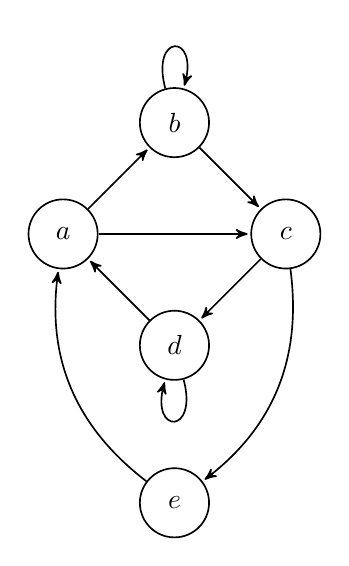
\begin{tikzpicture}[->,>=stealth',shorten >=1pt,auto,node distance=2cm,
                    semithick]
  \tikzstyle{every state}=[]

  \node[state] (A)                    {$a$};
  \node[state]         (B) [above right of=A] {$b$};
  \node[state]         (D) [below right of=A] {$d$};
  \node[state]         (C) [below right of=B] {$c$};
  \node[state]         (E) [below of=D]       {$e$};

  \path (A) edge              node {} (B)
            edge              node {} (C)
        (B) edge [loop above] node {} (B)
            edge              node {} (C)
        (C) edge              node {} (D)
            edge [bend left]  node {} (E)
        (D) edge [loop below] node {} (D)
            edge              node {} (A)
        (E) edge [bend left]  node {} (A);
\end{tikzpicture}
\caption{An example of a digraph for a relation.}\label{fig:digraph}
\end{center}
\end{figure}


\end{example}

\begin{exercise}
Let $A=\{a,b,c\}$ and define $\sim=\{(a,a),(a,b),(b,c),(c,b),(c,a)\}$.  Draw the digraph for $\sim$.
\end{exercise}

\begin{exercise}
Let $A=\{1,2,3,4,5,6\}$  Define $|$ on $A$ via $x|y$ iff $x$ divides $y$.  Draw the digraph for $|$ on $A$.
\end{exercise}

When $X$ or $Y$ is infinite, it is not practical to draw a digraph.  However, you are familiar with the graphs of some relations involving infinite sets.

\begin{example}
When we write $x^2+y^2=1$, we are implicitly defining a relation.  In particular, the relation is the set of ordered pairs $(x,y)$ satisfying $x^2+y^2=1$.  In set notation:
\[
\{(x,y):x^2+y^2=1\}
\]
The graph of this relation in $\mathbb{R}^2$ is the standard unit circle.
\end{example}

\begin{exercise}
Define $\sim$ on $\mathbb{R}$ via $x\sim y$ iff $x\leq y$.  Draw a picture of this relation in $\mathbb{R}^2$.
\end{exercise}

\begin{definition}
Let $\sim$ be a relation on a set $A$.
\begin{enumerate}
\item $\sim$ is \textbf{reflexive} if for all $x\in A$, $x\sim x$ (every element is related to itself).
\item $\sim$ is \textbf{symmetric} if for all $x,y\in A$, if $x\sim y$, then $y\sim x$.
\item $\sim$ is \textbf{transitive} if for all $x,y,z\in A$, if $x\sim y$ and $y\sim z$, then $x\sim z$.
\end{enumerate}
\end{definition}

\begin{example}\
\begin{enumerate}
\item $\leq$ on $\mathbb{R}$ is reflexive and transitive, but not symmetric.
$<$ on $\mathbb{R}$ is transitive, but not symmetric and not reflexive.
\item If $S$ is a set, then $\subseteq$ on $\mathcal{P}(S)$ is reflexive and transitive, but not symmetric.
\item $=$ on $\mathbb{R}$ is reflexive, symmetric, and transitive.
\end{enumerate}

\end{example}

\begin{exercise}
Given a finite set $A$ and a relation $\sim$, describe what each of reflexive, symmetric, and transitive look like in terms of a digraph.
\end{exercise}

\begin{exercise}
Let $P$ be the set of people at a party and define $N$ via $(x,y)\in N$ iff $x$ knows the name of $y$.  Describe what it would mean for $N$ to be reflexive, symmetric, and transitive.
\end{exercise}

\begin{exercise}
Determine whether each of the following relations is reflexive, symmetric, or transitive.

\begin{enumerate}
\item Let $P_f$ denote the set of all people with accounts on Facebook.  Define  $F$ via $xFy$ iff $x$ is friends with $y$. 
\item Let $P$ be the set of all people and define $H$ via $xHy$ iff $x$ and $y$ have the same height.
\item Let $P$ be the set of all people and define $T$ via $xTy$ iff $x$ is taller than $y$.
\item Consider the relation ``divides" on $\mathbb{N}$.
\item Let $L$ be the set of lines and define $||$ via $l_1||l_2$ iff $l_1$ is parallel to $l_2$.
\item Let $C[0,1]$ be the set of continuous functions on $[0,1]$.  Define $f\sim g$ iff
\[
\int_0^1|f(x)|\ dx=\int_0^1|g(x)|\ dx.
\]
\item Define $\sim$ on $\mathbb{N}$ via $n\sim m$ iff $n+m$ is even.
\item Define $D$ on $\mathbb{R}$ via $(x,y)\in D$ iff $x=2y$.
\end{enumerate}
\end{exercise}

\end{subsection}

\end{section}

\end{document}